\newpage 
\section{Auswertung}

    \subsection{Wheatstonesche Brückenschaltung}
        Für die erste Messreihe werden die Widerstände so eingestellt, dass die Brückenspannung minimal wird. 
        Die aufgenommenen Widerstände finden sich in Tabelle \ref{tab:tab1}.\\
        Anhand der Gleichung 
        \begin{equation}
            R_x= R_2 \cdot \frac{R_3}{R_4}\; \; ,
            \label{eqn:R}
        \end{equation}
        \noindent
        lässt sich der zu untersuchtende Widerstand $R_x$ des Bauteils \enquote{Wert 12} bestimmen.\\
        \begin{table}[ht]
          \centering
          \caption{Messwerte der Wheatstoneschen-Brückenschaltung}
          \label{tab:tab1}
          \begin{tabular}{S [table-format=3.0] S [table-format=3.0] S [table-format=3.0] S [table-format=3.2]}
           \toprule
            {$R_2 \mathbin{\scalebox{1.5} / } \si{\ohm}$} & {$R_3 \mathbin{\scalebox{1.5} / } \si{\ohm}$} & {$R_4 \mathbin{\scalebox{1.5} / } \si{\ohm}$} & {$R_x \mathbin{\scalebox{1.5} / } \si{\ohm}$}\\
           \midrule
           332 & 542 & 448 & 392.90 \\
           665 & 370 & 630 & 389.96  \\
           \bottomrule
          \end{tabular}
        \end{table} 
        Der Theoriewert von \enquote{Wert 12} beträgt $R_x= \SI{392.9}{\ohm}$.


    \subsection{Kapazitätsmessbrücke}
        Bei der Kapazitätsmessbrücke waren für das Bauteil \enquote*{Wert 9} der unbekannte Widerstand $R_x$
        und die unbekannte Kapazität $C_x$ zu bestimmen. Dabei wurde wieder das Minimum des Brückenstroms herbeigeführt.\\
        Mit Hilfe der Bauteildaten
        \begin{align*}
          R_2 = \SI{502}{\ohm}\\
          R_3 = \SI{451}{\ohm}\\
          R_4 = \SI{549}{\ohm}\\
          C_2 = \SI{399}{\nano\farad}\\
        \end{align*}
        lässt sich über Gleichung \ref{eqn:R} der Widerstand zu $R_x=\SI{413.21}{\ohm}$ berechnen.\\
        Über
        \begin{equation}
            C_x=C_2 \cdot \frac{R_4}{R_3}
            \label{eqn:C}
        \end{equation}
        ergibt sich $C_x=\SI{485.70}{\nano\farad}$.\\
        Die dazugehörigen Theoriewerte sind 
        \begin{align*}
          R_{x, Theo} &= \SI{413.2}{\ohm}\\
          C_{x, Theo} &= \SI{483.7}{\nano\farad}\; \; \text{.}
        \end{align*}


    \subsection{Induktivitätsbrückenschaltung}
        Bei dieser Brückenschaltung werden zu dem Bauteil \enquote{Wert 18}, der Widerstand $R_x$ und die Induktivität $L_x$ berechnet.
        Dafür wird für $R_x$ die Gleichung \ref{eqn:R} genutzt. Die Induktivität lässt sich mit
        \begin{equation}
            L_x=L_2 \cdot \frac{R_4}{R_3}
            \label{eqn:L}
        \end{equation}
        bestimmen.
        \begin{align*}
          R_2 = \SI{104}{\ohm}\\
          R_3 = \SI{775}{\ohm}\\
          R_4 = \SI{225}{\ohm}\\
          L_2 = \SI{16.6}{\milli\henry}
        \end{align*}
        Aus diesen ergeben sich für \enquote{Wert 18} für $R_x = \SI{358.22}{\ohm}$ und $L_x =\SI{4.82}{\milli\henry} $.

    \subsection{Maxwell-Brücke}
        Hier wird ein Bauteil auf seine Induktivität und seinen Widerstand untersucht. Die genutzten Bauteile besitzen folgende Spezifika:
        \begin{align*}
          R_2=1000\si{\ohm}\\
          R_3 = 64 \si{\ohm}\\
          R_4 = 638 \si{\ohm}\\
          C_2 = 399 \si{\nano\farad}
        \end{align*}
        Über Gleichung \ref{eqn:R} ergibt sich $R_x=\SI{100.31}{\ohm}$.\\
        Die Induktivität des Bauteils lässt sich über den Zusammenhang $L_x=C_2 R_3 R_4$ zu $L_x=\SI{25.536}{\milli\henry}$ bestimmen.
        Die damit korrespondierenden Theoriewerte sind
        \begin{align*}
            R_{x, Theo} &= \SI{108.7}{\ohm}\\
            L_{x, Theo} &= \SI{26.9}{\milli\henry}\; \; \text{.}
          \end{align*}

    \subsection{Wien-Robinson-Brücke}
        Mit den Widerständen $R=1 \si{\kilo\ohm}$, $R'=332 \si{\ohm}$ und einer Kapazität von $C = 399 \si{\nano\farad}$
        wurden für die Frequenzabhängigkeit der Spannungen in dieser Schaltung, die in Tabelle \ref{tab:tab2} aufgetragenen Werte, gemessen.
        Diese sind, inklusive Theoriekurve, auch in Abbildung \ref{img:plot1} zu finden.\\
        Für die Messreihe wurde eine konstante Spannung von $U_0=\SI{10}{\volt}$ angelegt.
        \begin{table}[ht]
          \centering
          \small
          \caption{Messdaten zur Wien-Robinson-Brücke}
          \label{tab:tab2}
          \begin{tabular}{S [table-format=5.0] S [table-format=1.3]}
           \toprule
           {$\nu \mathbin{\scalebox{1.5} / } \si{\hertz}$} & $\text{Amplitude} \mathbin{\scalebox{1.5} / } \si{\volt}$\\
           \midrule
           20 & 3.2   \\
           100 & 3     \\
           200 & 2     \\
           300 & 1.35  \\
           400 & 0.64  \\
           420 & 0.56  \\
           440 & 0.44  \\
           460 & 0.34  \\
           480 & 0.25  \\
           500 & 0.16  \\
           510 & 0.12  \\
           520 & 0.08  \\
           530 & 0.044 \\
           540 & 0.005 \\
           550 & 0.036 \\
           560 & 0.08  \\
           570 & 0.12  \\ 
           580 & 0.15  \\
           590 & 0.18  \\
           600 & 0.22  \\
           620 & 0.28  \\
           640 & 0.36  \\
           660 & 0.44  \\
           680 & 0.5   \\
           700 & 0.56  \\
           800 & 0.8   \\
           900 & 1.05  \\
          1000 & 1.25  \\
          1500 & 2     \\
          2000 & 2.4   \\
          3000 & 2.7   \\
          4000 & 2.8   \\
          5000 & 2.9   \\
          7500 & 3     \\
         10000 & 2.9   \\
          \bottomrule
          \end{tabular}
        \end{table} 
        Die Grenzfrequenz dieses Aufbaus $\nu_0$ enstpricht hier
        \begin{equation*}
          \omega_0=\frac{1}{RC}=\SI{539.50}{\hertz}\;\; .
        \end{equation*}
        Für die Theoriekurve wird dann $\Omega=\frac{\nu}{\nu_0}$ aufgetragen, mit $\nu_0=\frac{\omega_0}{2 \pi}$.
        Die Funktion hat dabei folgende Form:
        \begin{equation*}
          \frac{U_{Br}}{U_0}=\sqrt{\frac{1}{9}\frac{(\Omega^2-1)^2}{((1-\Omega^2)^2+9\Omega^2)}}
        \end{equation*}
        Gegen die Messwerte aufgetragen ist sie in Abbildung \ref{img:plot1}.

        \begin{figure}
            \centering
            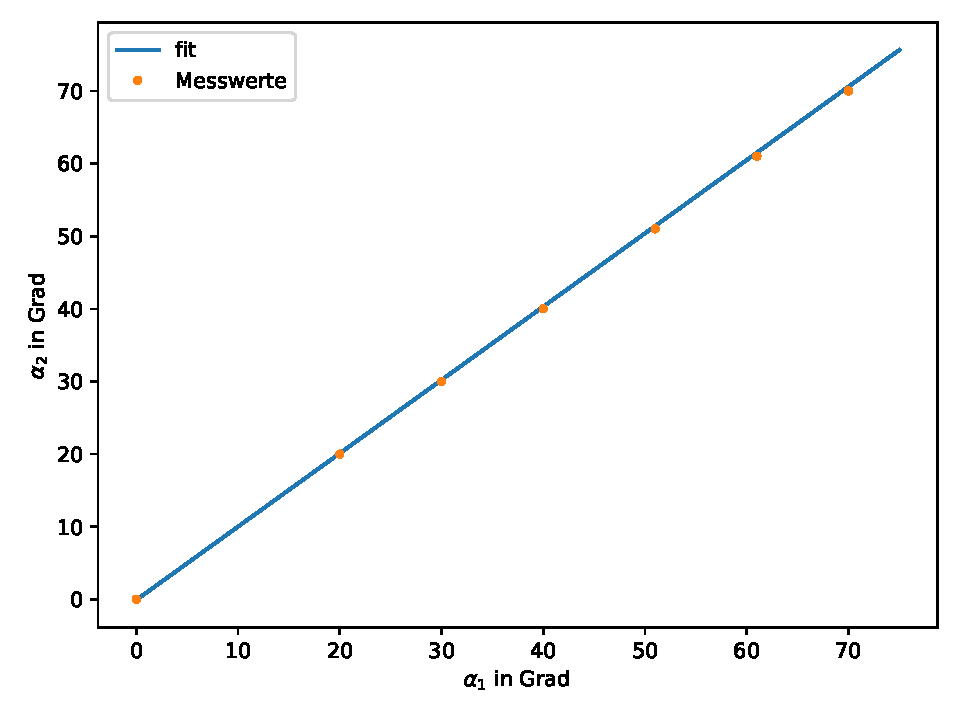
\includegraphics[width=0.6\textwidth]{build/plots/plot1.pdf}
            \caption{Messdaten zur Wien-Robinson-Brücke}
          \label{fig:plot1}
        \end{figure}
        \noindent
        Es ist zu sehen, dass die Messwerte und vorallem die Grenzfrequenz der Brückenspannung sich sehr gut mit der Theoriekurve decken. Nur für sehr hohe Frequenzen weichen sie leicht ab.\\ 
        Des Weiteren berechnet sich der Klirrfaktor des Sinusgenerators zu $k=3.35 \cdot 10^{-3}$.       